% THIS IS SIGPROC-SP.TEX - VERSION 3.1
% WORKS WITH V3.2SP OF ACM_PROC_ARTICLE-SP.CLS
% APRIL 2009
%
% It is an example file showing how to use the 'acm_proc_article-sp.cls' V3.2SP
% LaTeX2e document class file for Conference Proceedings submissions.
% ----------------------------------------------------------------------------------------------------------------
% This .tex file (and associated .cls V3.2SP) *DOES NOT* produce:
%       1) The Permission Statement
%       2) The Conference (location) Info information
%       3) The Copyright Line with ACM data
%       4) Page numbering
% ---------------------------------------------------------------------------------------------------------------

\documentclass{acm_proc_article-sp}
\usepackage[backend=biber,style=numeric]{biblatex}
\addbibresource{biblio.bib}
\addbibresource{Papers/SECURWARE/securware.bib}
\addbibresource{Papers/IMC -  Internet Measurement Conference/imc.bib}

\begin{document}

\title{CPSC 526 Final Report}
\subtitle{Tutorial Section: T02}
\date{\today}
\numberofauthors{3} 
\author{
\alignauthor
Stephen Dixon\\
       \email{sjdixon2@gmail.com}
\alignauthor
Kevin Chum\\
       \email{kchum@gmail.com}
\alignauthor
Rafael Benicio\\
       \email{rafaelbenicio2@gmail.com}
}

\maketitle

\begin{abstract}

\end{abstract}
\category{D3.3}{Operating System}{Security Protection}[Invasive Software]
\terms{Security}
\keywords{Malware, botnets, network security}

\section{Introduction}

Malware is one of the most serious threats facing the internet today, as it provides miscreants the means to perform a wide range of illegal and damaging activities, including distributed denial of service attacks, click fraud, data theft, and spam. According to McAfee and the Center for Strategic and International Studies, global cyber crime activity costs the world economy an estimated amount between \$300 billion and \$1 trillion dollars every year \cite{lewis:economics}.

Arguably, the most common form of malware today are bots; bots are programs which link compromised machines together in a command-and-control (C\&C) network; such networks, called botnets, allow botmasters to control and coordinate the bots by uploading payloads \cite{jacob:infiltration}.  Botnets used for a variety of purposes, such as fraud, theft, espionage, phishing, spam, and distributed denial of service attacks.

Botnets can be created in a variety of ways.  Some malware providers offer pay-per-installation services to help botmasters spread their programs \cite{caballero:distribution}.  Botnets can also be created through the use of a malicious proxy server which injects javascript code into web content using a man-in-the-middle attack; so-called javascript botnets are able to reach large audiences quickly and cheaply, but with reduced capability, as the malicious code is stored in the browser cache \cite{defcon:javascript}.

Botnets can communicate using a variety of channels.  Some botnets communicate over plain text, whereas other botnets employ their own proprietary cryptographic protocols to securely communicate between nodes \cite{stone:takeover}.  Botnets communicating to their botmasters via voice-over-IP (VOIP) have also been proposed \cite{defcon:voip} as well.  

Contemporary network security researchers have noticed that botnets are rapidly migrating from centralized server-based networks to peer-to-peer networks.  The reason for this migration is that peer-to-peer networks are more resilient against takeover, reconnaissance, and remediation efforts.  However, researchers have noted that most peer-to-peer botnets are actually hybrids \cite{defcon:prowling}, as botmasters still rely on centralized servers in order to collect the data collected by their bots.  Typically, such botnets consist of a modest number of relay nodes which serve as conduits between the central server and leaf nodes; many nodes, however, are actually unreachable by the botnet because they are located behind NAT networks, and must initiate contact with the bot server on their own. 

By establishing a systematic understanding of how botnets are structured and implemented, we can effective address and combat their effect on commerce and consumers. Despite the diversity of botnets on the internet, they often share similar purposes, and therefore share common challenges and design tradeoffs.  By design, botnets are meant to carry out their purposes in a coordinated, undetected, and unopposed manner, yet their need to communicate is the very thing that reveals and undoes them.


\section{Objectives}

In this paper, we investigate how botnets are purposed, designed, and implemented.  The paper is structured as follows: firstly, we discuss common design principles guiding the implementation of botnets, and how they vary in terms of their importance depending on the application; secondly, we discuss features implemented by botnets and the extent to which they lend themselves to the realization of the design principles.  

By design principles, we mean any principle or property of a system which allows a botmaster to effectively carry out the purpose of a botnet.  A typical botnet is designed like a bank robbery: first, the robbers must penetrate their target, then loot the valuables, and then make their getaway. In phishing, the purpose of the botnet is to spread word about a scam to unsuspecting victims. typically, the victims are tricked into purchasing objects like viagra, drugs, pills, or stock, or into giving away personal information or credit card information; these transactions are then exploited to defraud or rob the victims of their money
\cite{defcon:javascript}
\cite{defcon:spam}
\cite{wikipedia:phishing}.  On the other hand, trojan-horse botnets like Zeus collect sensitive information from victims through means such as keylogging, injecting web content into otherwise secure websites, and by granting attackers remote access \cite{defcon:javascript}
\cite{blackhat:zeus}
\cite{defcon:spam}
\cite{wikipedia:trojan}. Information and commands are relayed to and from the bots along a chain of relay nodes, which communicate with the control server through the use of a proxy server, which acts as a getaway car by anonymizing the server's identity.  In the VOIP botnet proposed by Itzik Kotler et. al of Security Art, a hacker could extract the stolen information simply by dialing into a conference call from a payphone anywhere in the world \cite{defcon:voip}.

By botnet features, we mean any protocol, algorithm, or process implemented by a bot program which realizes the purpose of the botnet.  Depending on the purpose of the botnet, bot programs may vary substantially.  For e

An important limitation of this paper is that the purpose, design, and implementation of criminal botnets are intentionally kept secret by their authors; consequently, we are limited to information which is publicly known. However, in some lucky cases, botnet authors do not implement secure features or protocols. Our sources include academic conferences such as USENIX, ACSAC,  and CCS, as well as black-hat conferences such as DEFCON.  We included non-traditional sources like DEFCON in order to get perspectives from botnet creators and the security industry, and to find cutting-edge botnet applications and implementation details, as we found that traditional academic sources did not have an insider's perspective on how botnets were created or implemented.

Centralized
Major Driver: Control
Major Weakness: Resilience

\section{How Infection is Implemented}
% How Bots Get Infected
    - how systems get infected

Bots are infected by specifics malwares that are responsible to cause damages using the most common attacks through email and drives-by downloads. By using email attachment some users can be attacked by someone because they do not pay attention this attachment is part of the attack. Email attachment is one of the most common attack used by attackers. Basically, the user is led to believe that the attachment contains safe information and it might be an important document such as bills. Instead, it contains malware that is activated as soon as the user opens the attachment. One relevant information is not a good practice of opening unknown files even if it is sent by a reliable person. For this specific attack, you can deselected the service to hide extensions from files. Then we can observe if there is a execution file or not. When the computer is part of the botnet when computer is infected.

There is another activity using malicious code such as drive-by downloads. For this specific attack, attackers load their malicious code into some websites with vulnerability securities and HTML tags that cause request to the victim's browser. Bots are compromised when malicious files are executed. 

Therefore, 

    - registration of new bots

One way how botmasters can register new bots is using attacks mechanisms to obtain new bots and collect information from users. Some Attackers have more expertise to propagate malicious code in computers because some people do not have much knowledge about it. By using tools and methods we observed how easily people can create a new botnet and how it can become a huge global market. People use to work with botnets because its part of their business as well as they can get millions of dollars working with. They can sell bots and also they can get bot from another botnet. Therefore, vulnerables systems and tools are used to exploit where bots are located and gain backdoor access to these systems becoming easier execution of bot malware by uploading or commanding the victim computer. People use to do direct and indirect techniques to spread an infected bot.  Peer-to-peer is also used to propagate malwares. Bot Malware uses HTTP, IRC protocol and can be created by other botnets. 

    - avoiding detection by anti virus
\subsection{Avoiding Detection by Antiviruses}
Because the main method through which botnets propagate is by malicious code, they must have methods to thwart antivirus utilities. Otherwise they would be detected and rendered unable to infect a target machine. 

In the event that a protected computer does manage to become infected and join the botnet --- for example if the strain of malware has not yet been detected by security companies --- then the malware may be able to kill any antivirus process that might be running, and block access to the vendor's website \cite{barford:book}. This might be done by editing the HOSTS file on Windows machines, or through the interception of packets being sent from or received by the infected machine. For botnets that have become widely known in the industry, this method becomes unfeasible without more sophisticated tactics.

The key weakness in most antivirus tools is that they work by comparing scanned binaries to a list of known malware signatures. Botnet creators take advantage of this property by writing malware that does not have a consistent signature. For example, the Storm botnet had multiple variants with different signatures that were released at certain intervals in order to circumvent antivirus scanning. By applying this principle on a large scale, botnet creators are able to easily stay ahead of antivirus updates. This technique is also known as \emph{serial variant evasion} \cite{ollmann:evasion}. There are several ways that new signatures can be generated, and these methods can be combined together to make an even larger set of possible signatures.

Metamorphic code (and also polymorphic code) is one method through which botnets can avoid antiviruses. The virus changes the 'look' of the binary without changing the semantics and overall meaning. This can be done, for example by exchanging two instructions where order does not matter, or by changing way the code achieves its purpose: using different registers or using different instructions to achieve the same thing. For instance in x86 assembly code, the instruction \texttt{xor eax eax} is syntactically different but causes the same end result as \texttt{mov eax 0}. Malware employ this method during propagation in order to have a different looking signature at each infection, thus circumventing any signature-based antivirus detection.

Another way to change the signature of malicious code is to add redundant or useless data, known as noise. This can be done either in the actual code of the malware or in its binary. In the code, a malware author can include constructs that essentially do nothing, for example testing if $1=1$, performing an arithmetic calculation without placing it in a variable, or adding NOPs. They can also write functions or add variables that are not actually used by the program. One last method is to add code routines that logically will not occur. For noise insertion to binaries, the programmer can add (possibly non-interpretable) data to the beginning or the end of the binary. Usually the malicious code itself is not modified. This insertion of garbage also has the added benefit that the malware producer can expand the malicious file to any arbitrary size that is desired, for example to match the filesize of some known benign file that is shared publicly, say in a torrent.

One more method that allows for changing virus signatures is to change how the compiler works on the code. Different compilers, versions of compilers, and settings used in compilation can drastically change how the final binary appears. In fact, some malware vendors utilize some automation frameworks like scripts to automatically change compilation variables \cite{ollmann:evasion}. However there is a caveat with this method: there are only so many ways to tweak settings in order to produce a new binary. Thus this method is not often seen on its own and instead combined with other techniques.



    % avoiding reverse engineering by sniffers, debuggers, honeypots etc.
\subsection{Avoiding Reverse Engineering by Sniffers, Debuggers, and Honeypots}


\section{How Command and Control is Traditionally Implemented}
% Evolution of Command & Control
    % single point of access (admin console)
    % communication channels for propagating commands/updates
% IRC, HTTP, HTTPS, encryption
% gossip protocols
% minimizing traffic footprint
% unreachable nodes
    % execution of commands?


When creating botnets, one major design decision lies in how bots are connected to each other and to the botmaster. Changes to this property can affect the amount of control over bots and the flow of data across the botnet. As of the time of writing, there are two major ways that botnets can be structured: as a centralized command and control (C\&C) infrastructure, or as a distributed peer-to-peer (P2P) network.  

In a command and control botnet, there is some central server where a botmaster can send commands to bots. Individual bots can also send any obtained data to this server, in the case that the botnet's malicious payload includes spyware. There are many C\&C botnets that use existing protocols as the base for their network, for example one prominent service is the Internet Relay Chat (IRC) protocol. However others may utilize HTTP as the underltying method to communicate with the server, such as the Asprox botnet \cite{borgaonkar:analysis}. 

Of the botnets that use IRC, Rajab et al. noted in 2006  \cite{rajab:botnets} that there were four prominent substructures. The first is the simplest and most widely used, where all bots connect to a single chat server. This structure has the disadvantage that the server capacity was often reached. To combat this problem and to support larger botnets, another structure is used where multiple IRC servers are linked together to form a network that has higher capacities. These botnets are known as \emph{bridged botnets}. Another method that is used by botmasters is to have several botnets that appear distinct but can be deduced to (via analysis of naming conventions and user IDs) be likely to belong to the same botmaster. The final observed structure is one where a subset of bots in one server are made to download a new binary that moves them to a different server.

Due to the prominence of IRC as a method for botnets to communicate, some corporations are beginning to block ports related to the protocol. As such, current trends in botnet communication appears to indicate a move towards more commonly seen protocols such as HTTP, or otherwise towards P2P networks.

Similar to the presence of multiple substructures for IRC-based botnets, Ollmann characterized C\&C botnets in general into several topologies \cite{ollmann:topology}, some of which appear to have counterparts to the IRC substructures. One of these is called the \emph{Star topology}. In this setup, each bot communicates directly with a single, centralized C\&C server. Another topology, similar to the idea of bridged botnets, is the multi-server C\&C topology. As the name implies, this method introduces several servers that act as command and control servers to the botnet. Another structure that Ollmann mentions is the hierarchical topology, in which bots are organized in a hierarchy and bots that are higher up can issue commands to bots further down in the tree.

Centralized command and control structures are attractive due to the fact that there is a single point of access for a botmaster, for instance through some web browser-based admin console. Through this point, they can command botnets to download new payloads, launch certain attacks or scans, or propagate on their network. For example, the Zeus botnet comes with a browser-based control panel, where botmasters can send new rules to, or collect data from bots. Using this application, they can also group different bots together and name them individually \cite{blackhat:zeus}. For IRC-based botnets, commands are typically made by setting the channel topic to some string recognized by the bots to be a command \cite{honeynet:appendix}. In both cases the botmaster still has to authenticate themselves to the bot, typically by providing a password. Botnets that use HTTP or HTTPS work in a similar way to those that are IRC-based: they poll a C\&C web server while waiting for new commands to be received \cite{borgaonkar:analysis}.

Another form of communication that is utilized by botnets are \emph{gossip protocols}. This kind of protocol relies on nodes passing on information that is learned to other nodes, thereby propagating it throughout the network. Gossip protocols are employed by peer-to-peer botnets \cite{defcon:prowling}, but can be utilized by hierarchical command and control botnets as well. Due to the need for communication to spread by nodes, the propagation speed is usually slower than direct messaging. However in larger botnets, this reduces the strain on the central C\&C server by delegating the command passing to other bots.


\section{The Getaway Car: How Data is Exfiltrated}
Evolution of Collection/Anonymity (the getaway car)
    - anonymity (tor, proxy servers, voip)
    - location (fast flux, voip)
    - how is communication different when sending info back to server?

Once data has been collected by bots, the process of exfiltrating the data back to the botmaster for monetization begins.  


\section{The Rise of Peer-to-Peer Botnets}

Contemporary botnets like ZeroAccess, MinerBot, Zeus, and Storm have adopted hybridized network structures in an effort to combine the resilience of peer-to-peer networks with the controllability of centralized servers.  Centralized servers are easy to construct, but have a single point of weakness: the command and control server itself \cite{wang:p2p}.  The nature of the network topology is surprisingly similar between peer-to-peer botnets;  ~\ref{fig:p2p-architecture} outlines the topology of peer-to-peer networks found in the likes of botnets such as ZeroAccess, MinerBot, Zeus, Storm, Conflicker, and Kelihos.

\begin{figure}[h]\centering
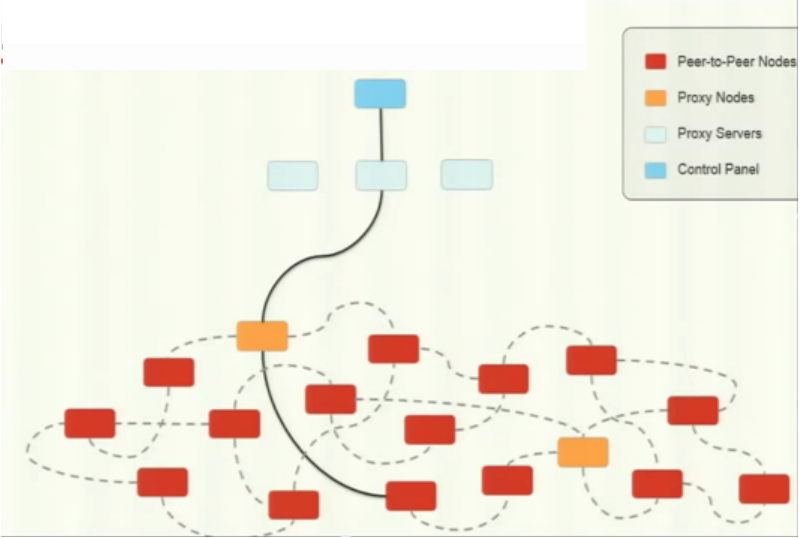
\includegraphics[width=0.45\textwidth]{p2p-architecture.png}
\caption{Peer-to-Peer Botnet Topology}
\label{fig:p2p-architecture}
\end{figure}


When individual bots want to receive commands from the botmaster, they send a request to some central components, through the use of peers, proxy nodes, and proxy servers. There is usually a layer of proxy servers being used, in order to provide redundancy in case they are taken down. Relaying requests in this manner helps disguise the location of the bot server on the internet \cite{defcon:prowling}.

Individual bots maintain a list of peers, obtained by communicating with other bots in the network.  In the ZeroAccess protocol, the peer list consists of a list of IP addresses and a timestamp indicating how recently the bot was active; the list was sorted in order of how recently the bot was active. In version 1 of the protocol, the peer list was 256 bots long and would bots that have not been active recently; in version 2, the peer list is 16 bots long and showed bots only if they were active recently.  It was suggested that the length of the peer lists were trimmed in order to reduce the traffic footprint of the botnet, as the botnet grew in size  \cite{defcon:prowling}.  

However, not all bots in the peer list are reachable.  Bots can be unreachable for a variety of reasons, such as being located inside NAT networks, or due to IP address churn.   Consequently, P2P botnets rely extensively on nodes which can be reached from anywhere; these nodes form the backbone of the botnet because of their positioning \cite{defcon:prowling}.

Message gossiping is utilized to propagate information\cite{stone:p2p}. A gossip protocol is a protocol in which a bot, in response to receiving information from another bot, forwards it to their peers. Each botnet uses customized message types and gossip protocols. For example, the Zeus botnet has the following message types:\cite{zeus:protocol}
\begin{itemize}
\item version request and reply - to determine a bot's current binary and configuration file\cite{zeus:protocol}.
\item peer list request and reply - to determine who the bot communicates with\cite{zeus:protocol}.
\item data request and reply - used to pull updates to the Zeus bot's binary or configuration files via UDP\cite{zeus:protocol}.
\item Proxy Reply - a signed message containing a list of proxies returned sent in response to a version request with some piggybcaked proxy request markers\cite{zeus:protocol}.
\item Proxy Announcement - a message announcing that a bot has been appointed as a proxy by the botmasters.  This message is then forwarded to the peer list of the bots who received the message.  To minimize the traffic footprint, this message type includes a time-to-live field which is decremented each time the message is forwarded; after reaching 0, bots do not forward the announcement any further\cite{zeus:protocol}.
\item C2 Message Type - a specialized, encrypted message exchanged between harvester bots and proxies, exchanged over HTTP and TCP protocols.  C2 message requests are sent by harvester bots to inform the server of the type of information harvested by the bot; the reply allows Zeus to tell the bot what to do with the information\cite{zeus:protocol}.
\end{itemize}

Research into peer-to-peer botnets has yielded a number of useful techniques for reconnaissance and disruption.  Reconnaissance is aimed at determining the size, topology, and vulnerabilites of a botnet, whereas disruption techniques are aimed at shutting down the botnets for good.  Two common reconnaissance techniques are crawling and sensor injection.  Crawling techniques use the peer-list mechanism implemented by botnets to determine all peers within the network, and who they are connected to. A number of factors limit the accuracy of crawling techniques; these include IP churn, non-routable peer clusters, peers with multiple IP addresses, and the frequency with which bots communicate with other bots.  Sensor injection techniques count the number of peers in a botnet by using the researcher's own machine as a relay node; this has the same effect as crawling does, except that some previously unreachable nodes will communicate with the sensor node.  In both reconnaissance techniques, a final approximate figure for the size of the botnet is obtained when the number of bots counted by the crawler or sensor converges towards a specific value \cite{stone:p2p}\cite{defcon:prowling}.

Common disruption techniques include sinkholing (in which bots are redirected to an offensive machine called a sinkhole) and partitioning (which aims to split the botnet into unusable subnets) \cite{stone:p2p}.  A sinkholing attack consists of several steps:
\begin{itemize}
\item Sinkhole Announcement - the intended sinkhole is sent to as many peers as possible.
\item Node isolation - the attacker attempts to eliminate all edges in the P2P graph that do not point to the sinkhole, effectively isolating peers from each other.
\item Fallback Prevention - many botnets have mechanisms that allow the bots to communicate directly with the command and control center in the event of a sinkhole attack.  Attackers must somehow disable the fallback channel or prevent bots from entering their fallback mode.
\end{itemize}

Botnets in the wild have employed a number of defenses against sinkhole attacks.  For example, the Sality botnet uses a reputation scheme in which each bot keeps track of the reputation of its neighbouring peers; reputation is increased by correctly responding to requests, and decreased by incorrectly responding to requests. Peers shared their peer lists only with other machines with high reputation, and only allow peer list entries with low reputations to be overwritten. Stone Gross et. al reverse-engineered the protocol to the extent that they could create their own high-reputation node, and they found ways to poison existing high-reputation nodes by overwriting their port numbers \cite{stone:p2p}.

On the other hand, the Zeus network uses a different scheme to prevent and mitigate sinkholing. Zeus bots announce their presence by sending requests to other bots on their peer list; upon receiving a request, Zeus bots add the source to its peer list if it knows fewer than 50 peers.  Zeus accounts for IP churn by assigning unique IDs to each bot, and updating the IP address whenever it receives an update for the bot identified with an ID it knows about.  Zeus mitigates the effect of spoofing through the use of an automated IP-based blacklist, which blocks IP addresses with high request rates \cite{stone:p2p}.

Furthermore, botnets employ a wide variety of fallback mechanisms in the wild.  Zeus bots periodically verify their neighbours every few days; if the bot is unable to update itself or its configuration files for seven days, it attempts to obtain a fresh peer list by contacting a set of hardcoded IP addresses, or by using a domain generation algorithm to lookup an appropriate command and control server.  As a result of these mechanism, sinkholing operations against Zeus are only temporarily successful \cite{stone:p2p}.

Domain generation algorithms, also known as domain flux and fast flux, grant bots the ability to communicate directly with the central components of a botnet.  However, the critical issue with domain generation algorithms is that the botnet reverts back to a centralized, non-P2P network, meaning that, once again, the network's resilience depends on how long these central resources can last.  In the case of the Torpig botnet, researchers were able to reverse-engineer the fast flux algorithm and take control of the botnet for over ten days; \cite{stone:takeover}.




Major Driver: Resilience
Major Limitation: Control
Evolution of Topologies
    - peer list, backbone nodes, unreachable nodes
    - ip churn/crawling
    - security/system benefits
    -topology (overlays, structured)


Control
resist to take-over / ownership
collection / 
over net / file sharing (torrent equivalent?)
threats -> flooding

(2 pages)
definition, relevance, depth/breadth


\section{Conclusion}
%Conclusion (1 page)

%Properties - needs secure

1
% Technique
%small footprint
%validation
%quick to update
%xml, topology, (web vs tree)
%secure
%against takeover, analysis, penetration
%untraceable
%anonymity, P2P, getawaster 
%well-position
%browser, service vs memories
%availability
%independent, node autonomy 
%hidden
%anti- debugger, anti-sniffer, Anti anti Virus
%frustration
%admin privilege, user lockout, anti - honeyspot,  difficult to RR


\printbibliography{}

\end{document}